\section{Rigid Body Kinematics}

\subsection{Rigid bodies}
\blue{Complete in "Rigid bodies"}

\subsection{Rotating rigid bodies}
\blue{Complete in "Rigid bodies"}

\subsection{Rigid body velocity}
\blue{Complete in "Rigid bodies"}

\subsection{Constrained motion}
\blue{Complete in "Constraints and constrained motions"}

\subsection{Rigid body acceleration}
\blue{Complete in "Rigid bodies"}

\subsection{\red{Gears}}
\red{Include the information in Fig \ref{fig:GearsRecap}  as a broad introduction to the topic}

\begin{figure}[h!]
    \centering
    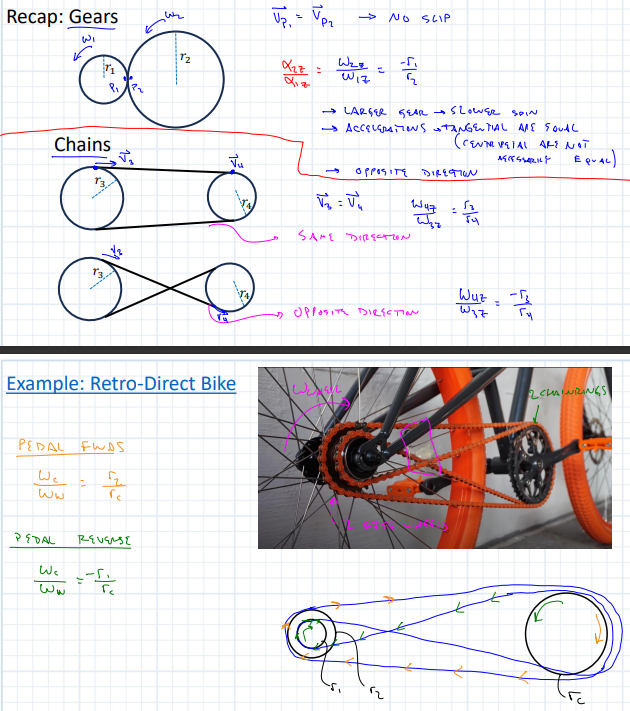
\includegraphics{RigidBodyKinematics/GearsRecap.png}
    \caption{From L21-Notes, slide 2}
    \label{fig:GearsRecap}
\end{figure}

    \subsubsection{\red{Standard sign convention}}
    \red{Add information shown in Fig \ref{fig:gears}}
    \begin{figure}[h!]
        \centering
        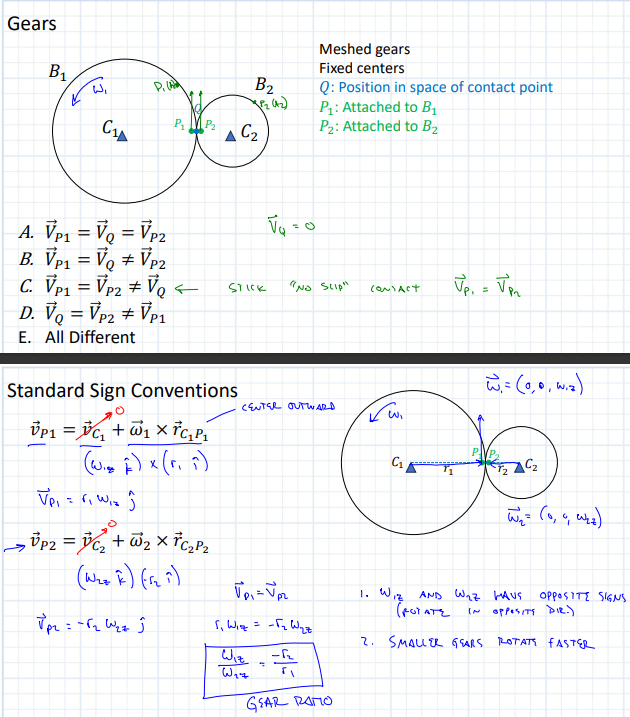
\includegraphics{RigidBodyKinematics/Gears.png}
        \caption{From L20-Notes, slides 4-5}
        \label{fig:gears}
    \end{figure}

\noindent \red{Include animation of examples as the ones in Fig \ref{fig:GearsExamples}}

    \begin{figure}[h!]
         \centering  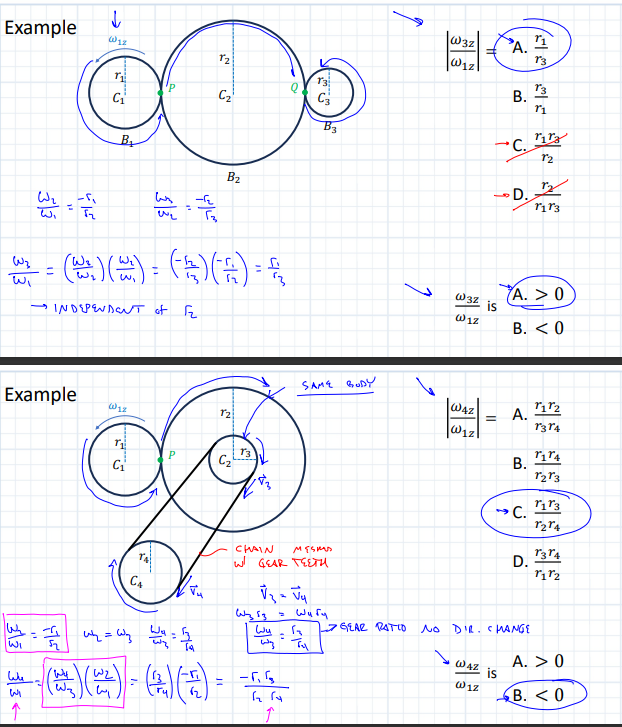
\includegraphics{RigidBodyKinematics/GearsExamples.png}    
         \caption{From L20-Notes, slides 7-8}
         \label{fig:GearsExamples}
    \end{figure}

    \subsubsection{\red{Accelerations in contact (no slip)}}
    \red{Add the information included in Fig \ref{fig:GearsAcceleration}}

    \begin{figure}[h!]
        \centering 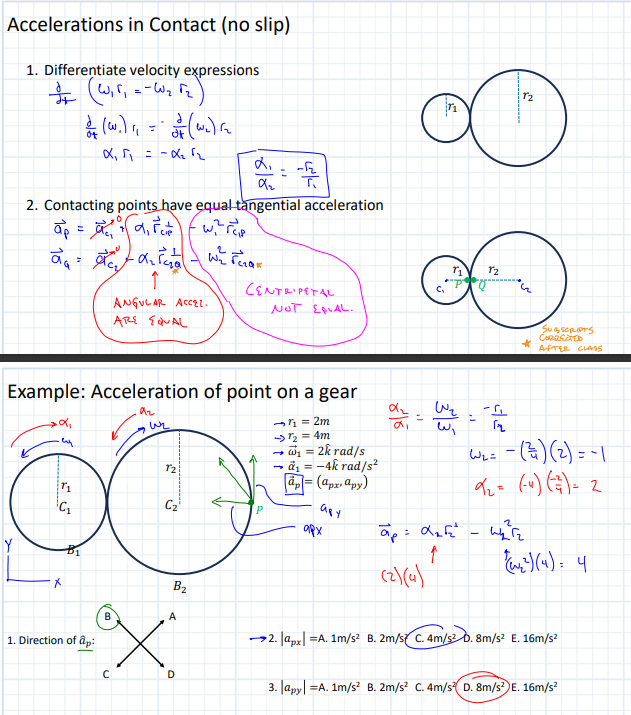
\includegraphics{RigidBodyKinematics/GearsAcceContact.png}
        \caption{From L20-Notes, slides 9-10}
        \label{fig:GearsAcceleration}
    \end{figure}
    
\subsection{\red{Applications}}
    \subsubsection{\red{Train passenger comfort}}
    \red{This topics need to be clearly organized and expanded. Refer to Fig \ref{fig:AppTrainPassenger}}. Application for "Rigid body acceleration".

    \begin{figure}[h!]
        \centering
        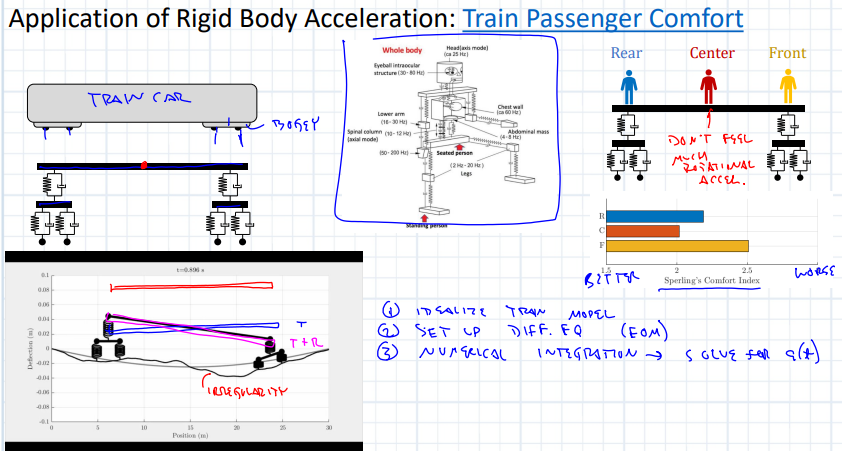
\includegraphics{RigidBodyKinematics/AppTrainPassenger.png}
        \caption{From L19-Notes, slide 2.}
        \label{fig:AppTrainPassenger}
    \end{figure}

    \subsubsection{Steering geometry}
    \blue{Complete in "Steering geometry".} This refers to "Rigid Bodies".

    \subsubsection{Knee Joint}
    \blue{Complete in "Four-Bar Linkages" under the subtitle "Example: Knee joint (constrained motion)".} This refers to "Constrained motion".

    \subsubsection{Suspensions with Watt's linkage}
    \blue{Complete in "Four-Bar Linkages" under the subtitle "Example: Suspensions with Watt's linkage (constrained motion)".} This refers to "Constrained motion".

    \subsubsection{\red{Aerobie Orbiter}}
    \red{This topic was mentioned in lecture but it was not expanded.} Application for "Rigid body rotation".

